

\chapter{TINJAUAN PUSTAKA}
\label{cha:2-TinjauanPustaka}

\section{Teorema Penaksiran Universal}
\label{sec:2-TeoremaPenaksiranUniversal}

Teorema penaksiran universal atau \textit{universal approximation theorem} menyatakan bahwa sebuah
model jaringan \textit{feed-forward} dapat membentuk fungsi apapun secara subjektif. Sebuah model
jaringan saraf tiruan dibentuk dari serangkaian lapisan yang didalamnya terdapat deretan sel saraf
atau \textit{neuron} dengan kuantitas tertentu. Semakin panjang rangkaian lapisan yang tersedia,
maka semakin banyak saraf yang tersedia sehingga dapat memetakan fungsi yang sulit.
Model jaringan yang memiliki banyak saraf dapat mempelajari pola-pola yang ada dari satu
domain ke domain lainnya~\cite{2016arXiv160100013G}.

Teorema penaksiran universal memiliki dua sifat yang dikategorikan berdasarkan pemanfaatannya dalam
melakukan pemelajaran mesin. Sifat pertama adalah suatu model jaringan saraf tiruan dapat
memperkirakan suatu fungsi dengan batasan-batasan tertentu sesuai dengan fungsi aktivasi pada
lapisan terakhir. Sifat kedua adalah sebuah fungsi kontinu dengan jumlah variabel sembarang dapat
ditiru oleh sebuah jaringan saraf tiruan dengan jumlah yang sembarang~\cite{2019arXiv191003344K}.

\section{Jaringan Saraf}
\label{sec:2-JaringanSaraf}

Otak manusia terdiri dari kumpulan sel saraf yang saling terkoneksi satu sama lain. Sebuah sel saraf
adalah sel yang dapat memproses dan mengantarkan informasi apabila dirangsang dengan tegangan
elektrokimia. Sel-sel saraf tidak pernah memperbanyak dirinya dan tidak digantikan apabila ada yang
rusak. Jumlah sel saraf yang terdapat dalam otak manusia diperkirakan sebanyak satu miliar. Setiap
sel saraf diperkirakan berkoneksi dengan sepuluh ribu sel saraf lainnya melalui sinapsis yang
berarti otak manusia beroperasi seperti prosesor dengan kecepatan satu triliun bit per
detik~\cite{10.3389/neuro.09.031.2009}.

\begin{figure}[htbp]
    \begin{center}
        \fbox{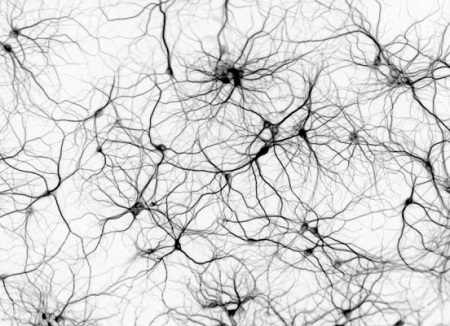
\includegraphics[scale=1.0]{bab2/gambar/jaringansaraf.jpg}}
    \end{center}
    \vspace{-20pt}
    \captionsetup{labelfont=bf, textfont=bf}
    \caption{Ilustrasi Jaringan Saraf Manusia}
    \vspace{-10pt}
    \captionsetup{labelfont=md, textfont=md}
    % \caption*{Sumber: https://upload.wikimedia.org/wikipedia/commons/b/b5/Neuron.svg}
    % \caption*{Sumber: Zhang (2019)}
    \label{fig:jaringansaraf}
\end{figure}

Bentuk sel saraf sangat bervariasi dengan berbagai ukuran, bentuk, dan sifat elektrokimianya. Sebuah
sel saraf memiliki badan yang terdiri dari beberapa struktur penting meliputi \textit{soma},
\textit{dendrites}, \textit{axon}, dan \textit{synapses} seperti pada gambar~\ref{fig:selsaraf}.
Sebuah sel saraf akan menerima beberapa masukkan melalui \textit{synapses}, memproses inputan
tersebut melewati \textit{dendrites}, kemudian diteruskan melalui \textit{soma}, dan diberikan
kepada sel saraf lainnya melalui \textit{axon}~\cite{2019arXiv190601703Z}.

\begin{figure}[htbp]
    \begin{center}
        \fbox{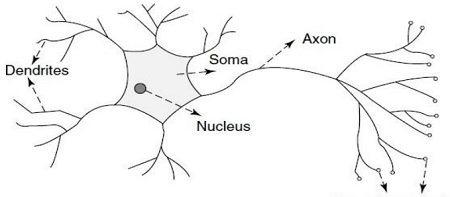
\includegraphics[scale=1.0]{bab2/gambar/selsaraf.jpg}}
    \end{center}
    \vspace{-20pt}
    \captionsetup{labelfont=bf, textfont=bf}
    \caption{Ilustrasi Sel Saraf Manusia}
    \vspace{-10pt}
    \captionsetup{labelfont=md, textfont=md}
    % \caption*{Sumber: https://upload.wikimedia.org/wikipedia/commons/b/b5/Neuron.svg}
    % \caption*{Sumber: Zhang (2019)}
    \label{fig:selsaraf}
\end{figure}

\section{Jaringan Saraf Tiruan}
\label{sec:2-JaringanSarafTiruan}

Jaringan Saraf Tiruan adalah sistem komputasi yang cara kerjanya menyerupai jaringan saraf pada otak
makhluk hidup. Tidak seperti pemrograman secara konvensional, sebuah jaringan saraf tiruan dapat
memodelkan fungsi sembarang yang tingkat kesulitannya sesuai dengan jumlah koneksi yang ada. Sama
seperti jaringan saraf asli, sebuah saraf tiruan juga menerima banyak masukkan dari saraf lainnya
kemudian dioperasikan dengan bobot yang terkadung pada sel tersebut dan akhirnya diteruskan ke sel
berikutnya. Jaringan saraf umumnya dibentuk kedalam beberapa lapisan seperti pada
gambar~\ref{fig:jaringansaraftiruan}~\cite{croann}.

\begin{figure}[htbp]
    \begin{center}
        \fbox{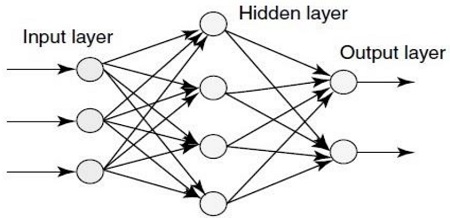
\includegraphics[scale=1.0]{bab2/gambar/jaringansaraftiruan.jpg}}
    \end{center}
    \vspace{-20pt}
    \captionsetup{labelfont=bf, textfont=bf}
    \caption{Ilustrasi Jaringan Saraf Tiruan}
    \vspace{-10pt}
    \captionsetup{labelfont=md, textfont=md}
    % \caption*{Sumber: https://upload.wikimedia.org/wikipedia/commons/b/b5/Neuron.svg}
    % \caption*{Sumber: Zhang (2019)}
    \label{fig:jaringansaraftiruan}
\end{figure}

Sebuah sel saraf saraf dapat dibagi menjadi empat bagian yang meliputi masukkan, bobot, fungsi
transfer atau aktivasi, dan keluaran. Jumlah masukkan pada suatu sel saraf tiruan berjumlah sebanyak
output dari sel-sel yang berada pada layer sebelumnya. Bobot sel adalah nilai numerik yang menjadi
identitas dari sel yang merupakan hasil penyesuaian dari proses latihan. Fungsi aktivasi adalah
sebuah fungsi menerima hasil operasi antara bobot dan masukkan. Keluaran merupakan hasil dari sel
yang diteruskan ke lapisan selanjutnya. Ilustrasi sebuah sel saraf tiruan dapat dilihat pada gambar
~\ref{fig:saraftiruan}~\cite{Sharma2012ACS}.

\begin{figure}[htbp]
    \begin{center}
        \fbox{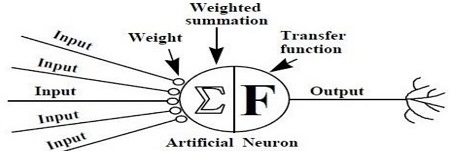
\includegraphics[scale=1.0]{bab2/gambar/saraftiruan.jpg}}
    \end{center}
    \vspace{-20pt}
    \captionsetup{labelfont=bf, textfont=bf}
    \caption{Ilustrasi Sel Saraf Tiruan}
    \vspace{-10pt}
    \captionsetup{labelfont=md, textfont=md}
    % \caption*{Sumber: https://upload.wikimedia.org/wikipedia/commons/b/b5/Neuron.svg}
    % \caption*{Sumber: Zhang (2019)}
    \label{fig:saraftiruan}
\end{figure}

\section{Fungsi Aktivasi}
\label{sec:2-FungsiAktivasi}

Fungsi aktivasi pada sel saraf tiruan berfungsi untuk mengkonversi hasil operasi matriks antara
masukkan dan bobot sebuah sel dari sistem linier ke sistem nonlinier. Konversi nilai ini dilakukan
agar setiap sel mengambil perannya pada saat proses pelatihan model. Beberapa fungsi aktivasi yang
dipakai pada umumnya adalah \textit{Sigmoid}, \textit{ReLU}, \textit{Tanh}, dan \textit{Softmax}
~\cite{2014arXiv1412.6830A}.

\textit{Rectified Linear Unit} adalah fungsi aktivasi yang paling umum digunakan dalam aplikasi
jaringan saraf tiruan. Fungsi aktivasi \textit{ReLU} membatasi nilai masukkannya dimana nilai yang
kurang dari nol akan diubah menjadi nol~\cite{Hinton_rectifiedlinear, 2018arXiv181103378N}.
Persamaan fungsi aktivasi \textit{Rectified Linear Unit} dapat dilihat seperti pada persamaan dibawah.

\begin{equation*}
    \;f(x)=\;max\left(0,x\right)=\;\left\{\begin{array}{l}x_{i,\;}\;\;if\;x_i\;\geq\;0\\0,\;\;\;\;if\;x_i<\;0\;\;\end{array}\right.\;\;
\end{equation*}

\begin{figure}[htbp]
    \begin{center}
        \fbox{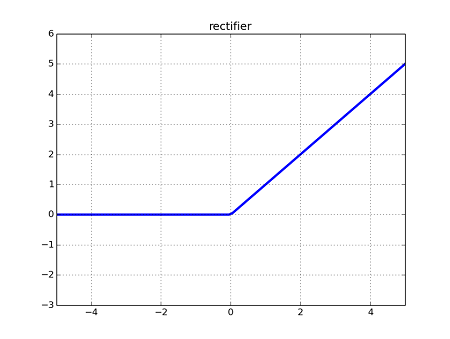
\includegraphics[scale=1.0]{bab2/gambar/relu.png}}
    \end{center}
    \vspace{-20pt}
    \captionsetup{labelfont=bf, textfont=bf}
    \caption{\textit{Rectified Linear Unit}}
    \vspace{-10pt}
    \captionsetup{labelfont=md, textfont=md}
    % \caption*{Sumber: https://upload.wikimedia.org/wikipedia/commons/b/b5/Neuron.svg}
    % \caption*{Sumber: Zhang (2019)}
    \label{fig:relu}
\end{figure}

\section{Residual Network}
\label{sec:2-ResidualNetwork}

\textit{Residual Network} atau \textit{ResNet} merupakan model jaringan saraf tiruan yang menggunakan \textit{residual block}
sebagai dasar dari setiap lapisan. Sebuah \textit{residual block} merupakan sebuah arsitektur jaringan
saraf tiruan kecil yang terdiri dari beberapa lapisan. Setiap blok akan menjumlahkan masukkan dan
keluarannya sehingga layer di dalam suatu blok hanya menambahkan pola-pola yang dipelajari. Hal ini
memungkinkan \textit{ResNet} untuk memiliki jumlah blok yang sangat banyak sehingga dapat memetakan
suatu fungsi sembarang yang sulit sesuai dengan teorema penaksiran universal~\cite{2015arXiv151203385H}.
Jenis-jenis \textit{residual block} dapat dilihat pada gambar~\ref{fig:resblock}.

\begin{figure}[htbp]
    \begin{center}
        \fbox{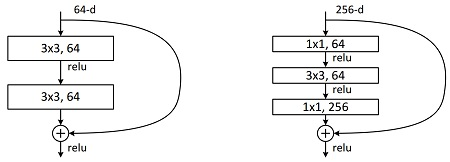
\includegraphics[scale=1.0]{bab2/gambar/resnet.jpg}}
    \end{center}
    \vspace{-20pt}
    \captionsetup{labelfont=bf, textfont=bf}
    \caption{\textit{\textit{Residual Block}}}
    \vspace{-10pt}
    \captionsetup{labelfont=md, textfont=md}
    % \caption*{Sumber: https://upload.wikimedia.org/wikipedia/commons/b/b5/Neuron.svg}
    % \caption*{Sumber: Zhang (2019)}
    \label{fig:resblock}
\end{figure}

\section{Optimisasi Model}
\label{sec:2-OptimisasiModel}

Algoritma optimisasi model yang paling populer dalam melakukan pelatihan model \textit{deep learning}
adalah \textit{gradient descent}. \textit{Gradient descent} meminimalisir selisih antara prediksi
model dan target sebenarnya dengan merubah bobot-bobot yang terdapat dalam model. Nilai bobot yang
ditambahkan berbanding terbalik dengan gradien hasil fungsi kesalahan terhadap masing-masing bobot.
Proses optimisasi dilakukan dengan melakukan \textit{forward-pass} dan \textit{backpropagation} yang
melibatkan beberapa elemen seperti \textit{learning rate}, \textit{optimizer},
dan \textit{loss function}. Tujuannya adalah untuk mencapai titik optimal pada sebuah bidang berdasarkan
hasil dari \textit{loss function}~\cite{2016arXiv160100013G}. Ilustrasi titik optimal digambarkan
pada gambar~\ref{fig:gradientdescent}.

\begin{figure}[htbp]
    \begin{center}
        \fbox{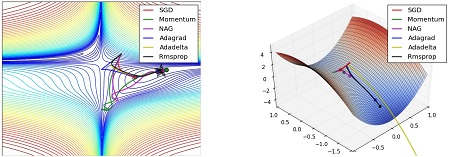
\includegraphics[scale=1.0]{bab2/gambar/gradientdescent.jpg}}
    \end{center}
    \vspace{-20pt}
    \captionsetup{labelfont=bf, textfont=bf}
    \caption{\textit{\textit{Gradient Descent}}}
    \vspace{-10pt}
    \captionsetup{labelfont=md, textfont=md}
    % \caption*{Sumber: https://upload.wikimedia.org/wikipedia/commons/b/b5/Neuron.svg}
    % \caption*{Sumber: Zhang (2019)}
    \label{fig:gradientdescent}
\end{figure}

lr, adam, loss function

\section{Estimasi Pose Dua Dimensi}
\label{sec:2-EstimasiPoseDuaDimensi}
citasi~\cite{8765346}

\section{Estimasi Pose Tiga Dimensi}
\label{sec:2-EstimasiPoseTigaDimensi}

citasi~\cite{martinez_2017_3dbaseline}

\section{PyTorch}
\label{sec:2-PyTorch}

pytorch dynamic graph

\begin{table}[htbp]
    \captionsetup{labelfont=bf, textfont=bf}
    \caption{Sebuah tabel}
    \vspace{-20pt}
    \begin{center}
        \begin{tabular}{| l c r |}
            \hline
            1 & 2 & 3 \\
            4 & 5 & 6 \\
            7 & 8 & 9 \\
            \hline
        \end{tabular}
    \end{center}
    \vspace{-10pt}
    \captionsetup{labelfont=md, textfont=md}
    \caption*{Sumber: Bego Lu}
\end{table}

